\chapter{Introduction}

\section{Like Astronomy, but Closer}

Space physics is a field of study that encompasses natural phenomena that occur in our own solar system. The basic difference between it, and the much older field of Astronomy, is that in-situ measurements and direct experiments are possible. As a separate field of study, space physics began in earnest at the beginning of the space age, with the flights of the first instrumented spacecraft. The discovery of the radiation belts that surround Earth was a profound example of the subsequently rapid increase in knowledge about the space surrounding Earth, which is a trend that has continued to the present day. At the same time, and equally importantly, ground based and remote sensing techniques have advanced to the degree that robust, distributed, measurements of the properties of the space around Earth are readily available. The synthesis of these two orthogonal, but complimentary, sources of data gives the field of space physics a distinct image among the sciences, and motivates its pursuit not just for its own sake, but as a window to the workings of the wider universe which we cannot reach.

Space physics is a field which, owing to its proximity to technologies which have become important to our society, has many useful applications. This is not, or at least, should not be, the primary motivation for its study. Scientific advancement, along with education in general, has garnered a reputation in recent western society, as simply a tool, to be used for the immediate improvement of our material lives. This is a dangerous, limited mindset, with implications that can extend far into the future. As we come to face the first of the extreme consequences of our way of life, humans will have to make choices which will affect the world for future generations. Informing these decisions from a utilitarian perspective will limit our view to the world as we live in it today, despite the fact that it is changing, and will continue to change, due to our actions. 

The typical return on investment, in an economic sense, for scientific progress, is measured in decades and sometimes centuries. Although exceptions exist, this is generally incompatible with a worldview centred completely on the present. Most of science is generational work, with contemporary efforts built upon those already accomplished by people who lived in different times. The view that this represents a problem which needs to be corrected, stems from the utilitarian view, and depends on the implicit assumption that our resources are limitless, and that uncontrolled, exponential growth of our society is sustainable. Recent events, including climate change driven natural disasters and the COVID-19 pandemic, provide a dramatic demonstration that this is false. 

Uncontrolled growth in technology and knowledge, without the human view that contributing to our shared knowledge is valuable, is prone to emphasizing negative applications. Nuclear science, artificial intelligence, and genetic engineering are all examples where the science has been drowned out, in popular discourse, by their worst uses. This has a suffocating effect on not only these fields, but the rest of scientific inquiry. A more rational view can help with this problem, by acknowledging the power scientific knowledge gives us, along with the fact that we, as humans, have a choice in how it is used. This view is not one which propagates well in an environment completely determined by utility. 

In the present time, we are contending with worldviews that are against science for its own sake, which in the end, is being against science in general. Coming back to a sane perspective, which admits that our human curiosity and collective knowledge has value, is going to be a difficult process. As an antidote to bigotry, nationalism, and zero-sum thinking focused only in the present, the attitudes encouraged by science may yet be what saves us. We need to work together, today, to advance science as being worthwhile. This thesis, like many others, is written to make a contribution in this spirit. 


\begin{figure}[p]
\label{keep_looking_up}
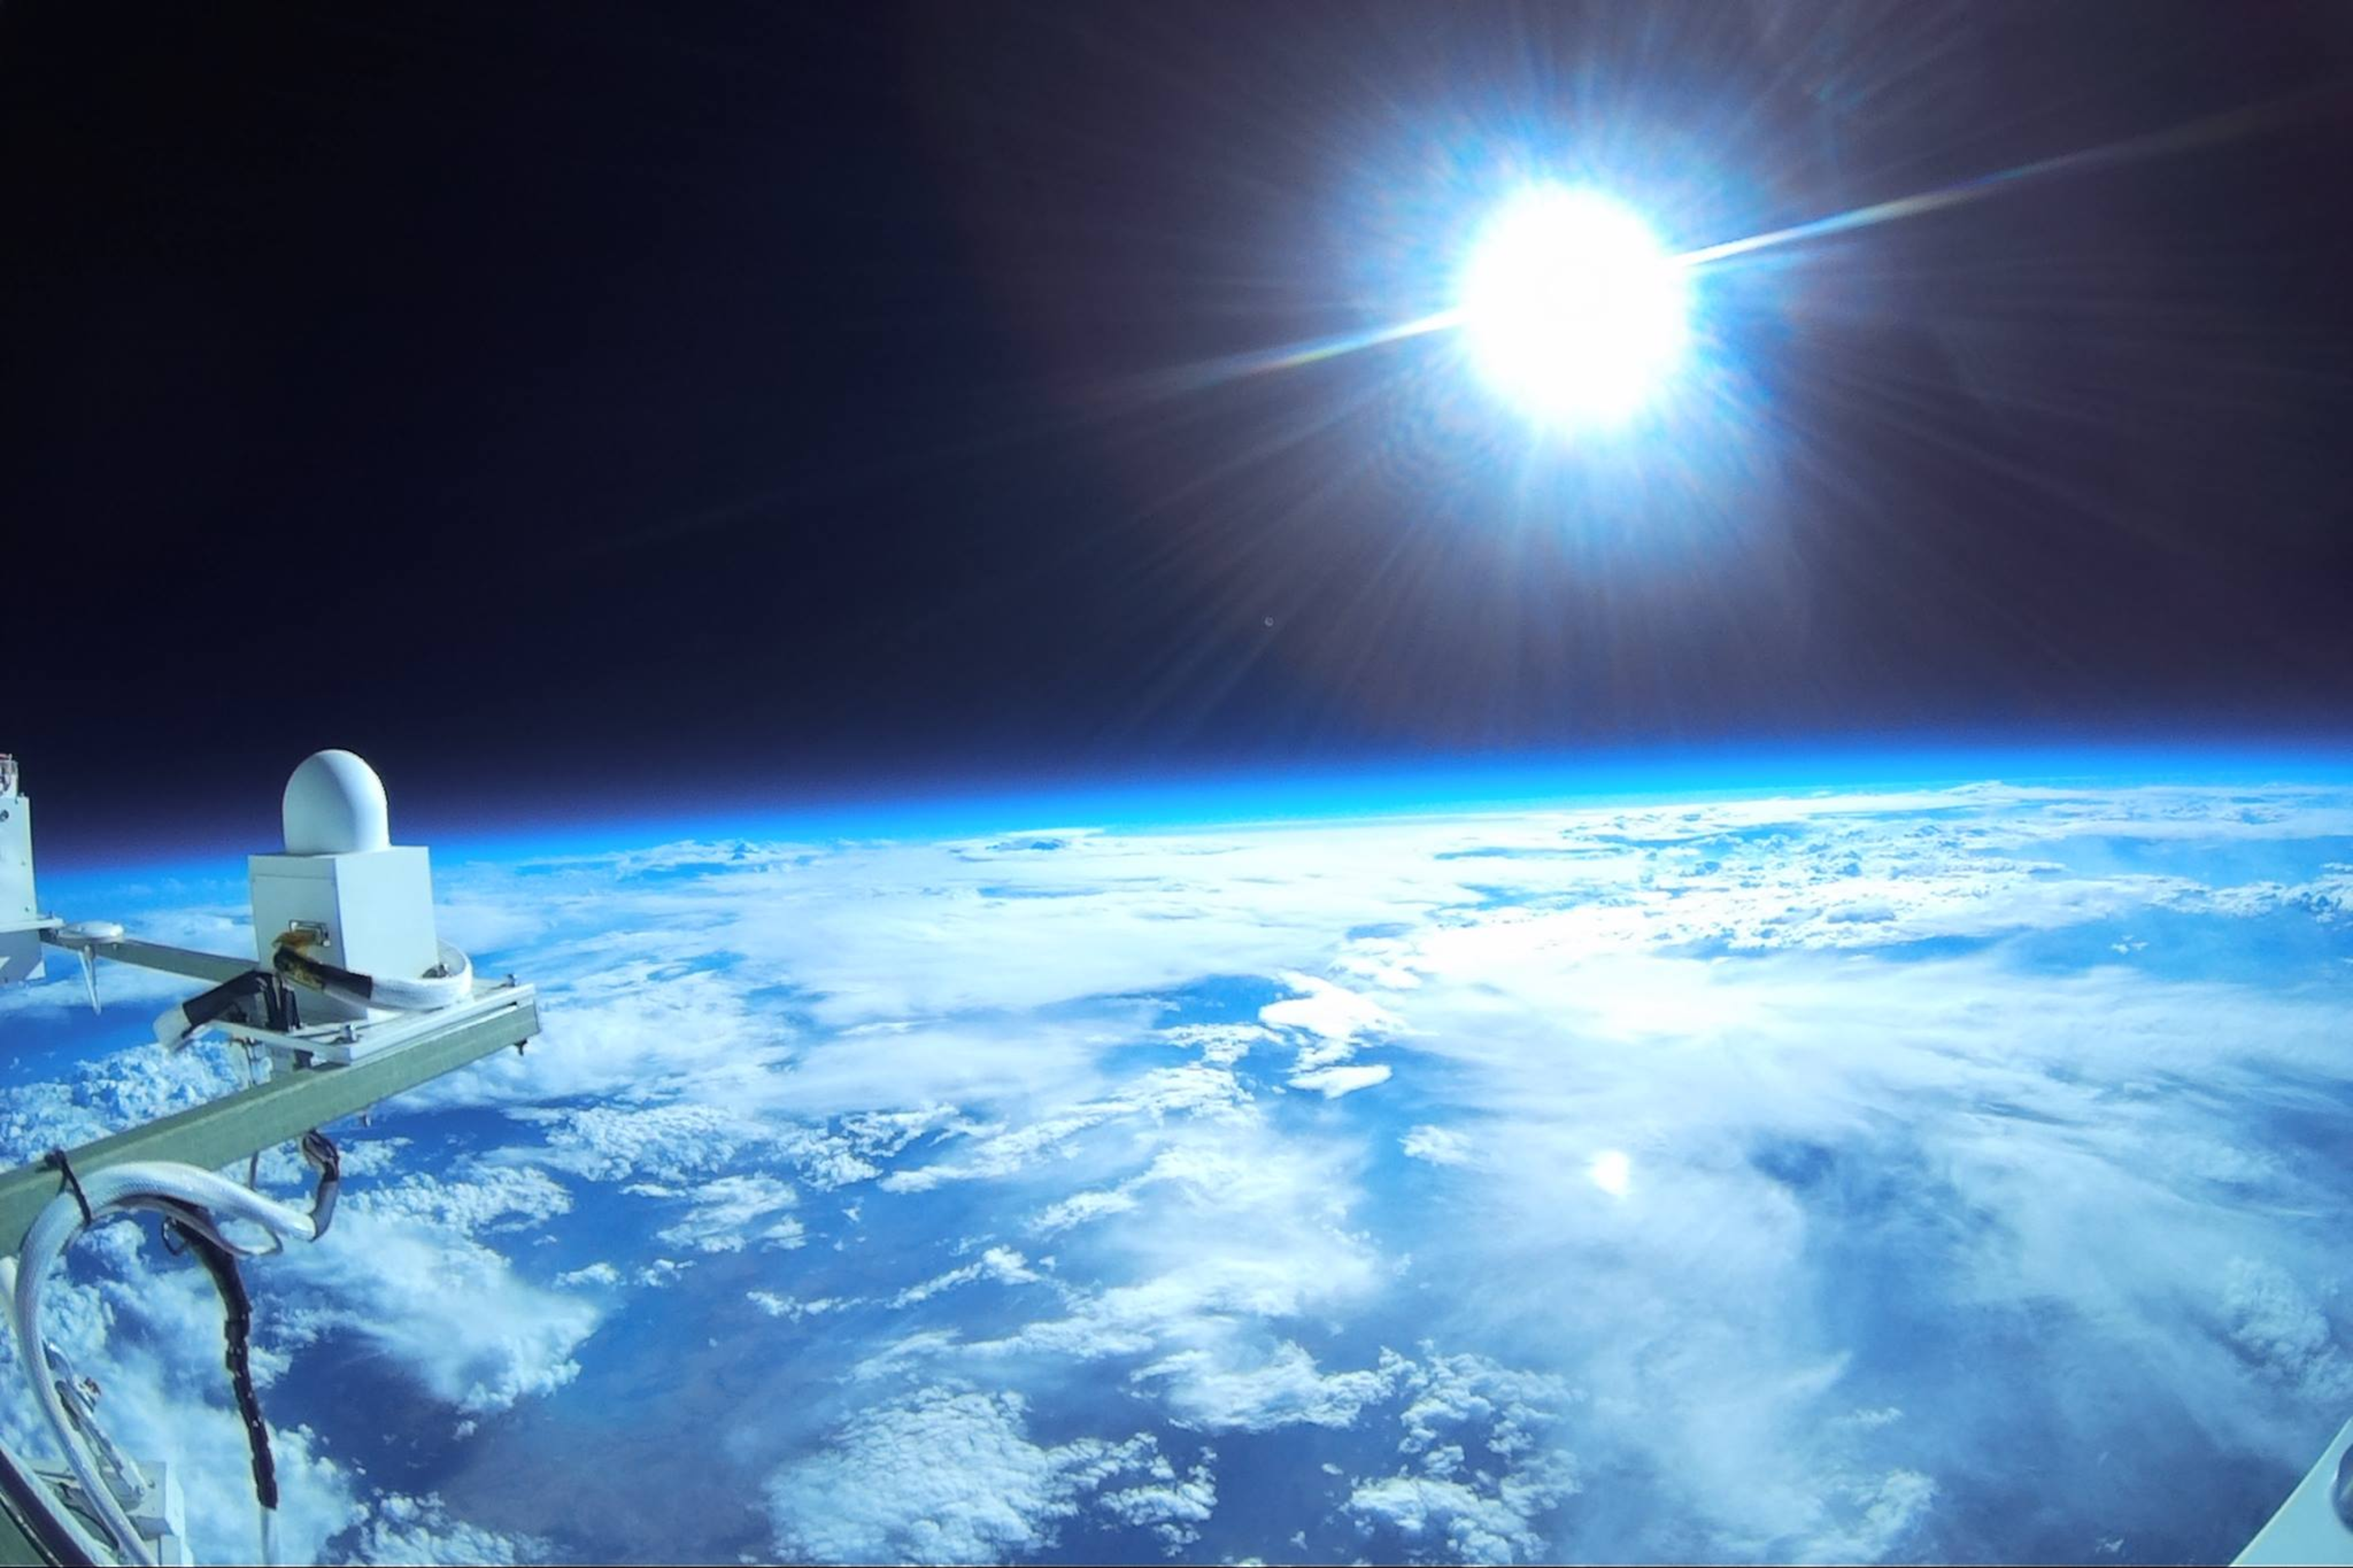
\includegraphics[width=\textwidth]{figures/chapter_1/keep_looking_up/keep_looking_up}
\caption{Picture taken by an instrumented balloon payload, built by secondary students and flown on the NASA HASP (high altitude student platform) flight in 2017. }
\end{figure}

\section{(Not So) Empty Space}

The space surrounding the Earth is full of activity. To get a picture of this, one only needs to look at the Aurora Borealis, one of the dramatic and beautiful manifestations of this system. When they occur, the aurora aren't static features. Depending on the type of aurora, they can present as shimmering curtains, pulsing patches, or diffuse regions. These types are not exclusive. Dynamic structures like these, in space and time, are often indicative of a complex system. The old myth - that the aurora are caused by the solar wind following the magnetic field of the Earth and hitting the atmosphere - falls flat in light of this complexity. In fact, the current state of knowledge paints a much different picture, with internal properties of the space and constituents surrounding Earth doing most of the ``work'' producing the aurora, which then carries much information about the entire system. 

There are two basic kinds of entity in near Earth space: fields, and particles, which may be electrically charged. Classical electromagnetism provides a sufficiently accurate description of these in most cases. These are them, in one of their most common forms:

  \begin{subequations}
    \begin{alignat}{2}
      \mathllap{\text{Gauss' Law}\qquad} && \nabla\cdot\mathbf{E} &= \frac{\rho}{\varepsilon_0} \\
      \mathllap{\text{Gauss' Law ($\mathbf{B}$ Fields)}\qquad} && \nabla\cdot\mathbf{B}  &= 0 \\
      \mathllap{\text{Faraday's Law}\qquad} && \nabla\times\mathbf{E} &= -\frac{\partial \mathbf{B}}{\partial t} \\
      \mathllap{\text{Ampere's Law}\qquad} && \nabla\times\mathbf{B} &= \mu_0\mathbf{J}+\mu_0\varepsilon_0\frac{\partial\mathbf{E}}{\partial t}
    \end{alignat}.
  \end{subequations}

In these equations, $\mathbf{E}$ and $\mathbf{B}$ are the electric and magnetic fields, $\mathbf{J}$ is electrical current, $\rho$ is charge density, and $\mu_0, \varepsilon_0$ are constants. These have been known for a long time, but they contain the root of why the space around Earth is a complicated place. When you have charged particles, they move according to electromagnetic fields, but while they move, they also affect the fields themselves. In an environment like near Earth space, where matter mostly exists as a plasma of charged particles, this gives rise to collective, or self-consistent behaviour and is a source of complexity. Further, a simple analysis of Maxwell's equations shows that wave phenomena also occur. This is combined with the fluid character that particles in large numbers display to make what is called plasma physics. 

Plasma is a name given to a state of matter which much of the material surround Earth exists in. It can be roughly defined as a gas of positive and negatively charged particles in approximately equal number, free to move, and at a high temperature. There is a more precise definition, which comes from statistical mechanics. In general, though, it is accurate to say that one of the defining characteristics of a plasma is the combination of the long-range electromagnetic interaction, with short-range collisional and fluid properties. Plasma waves, collective motion, and the propagation, absorption, and emission of radio waves are all observed in the space surrounding Earth. Based on all of this, the overall picture is not one of cold, dark, and empty space, but of a lively and energetic environment, constantly in motion and full of vibrations, with energy, matter, and information all flowing through the system. 

\begin{figure}[h]
\label{aurora_from_space}
\begin{centering}
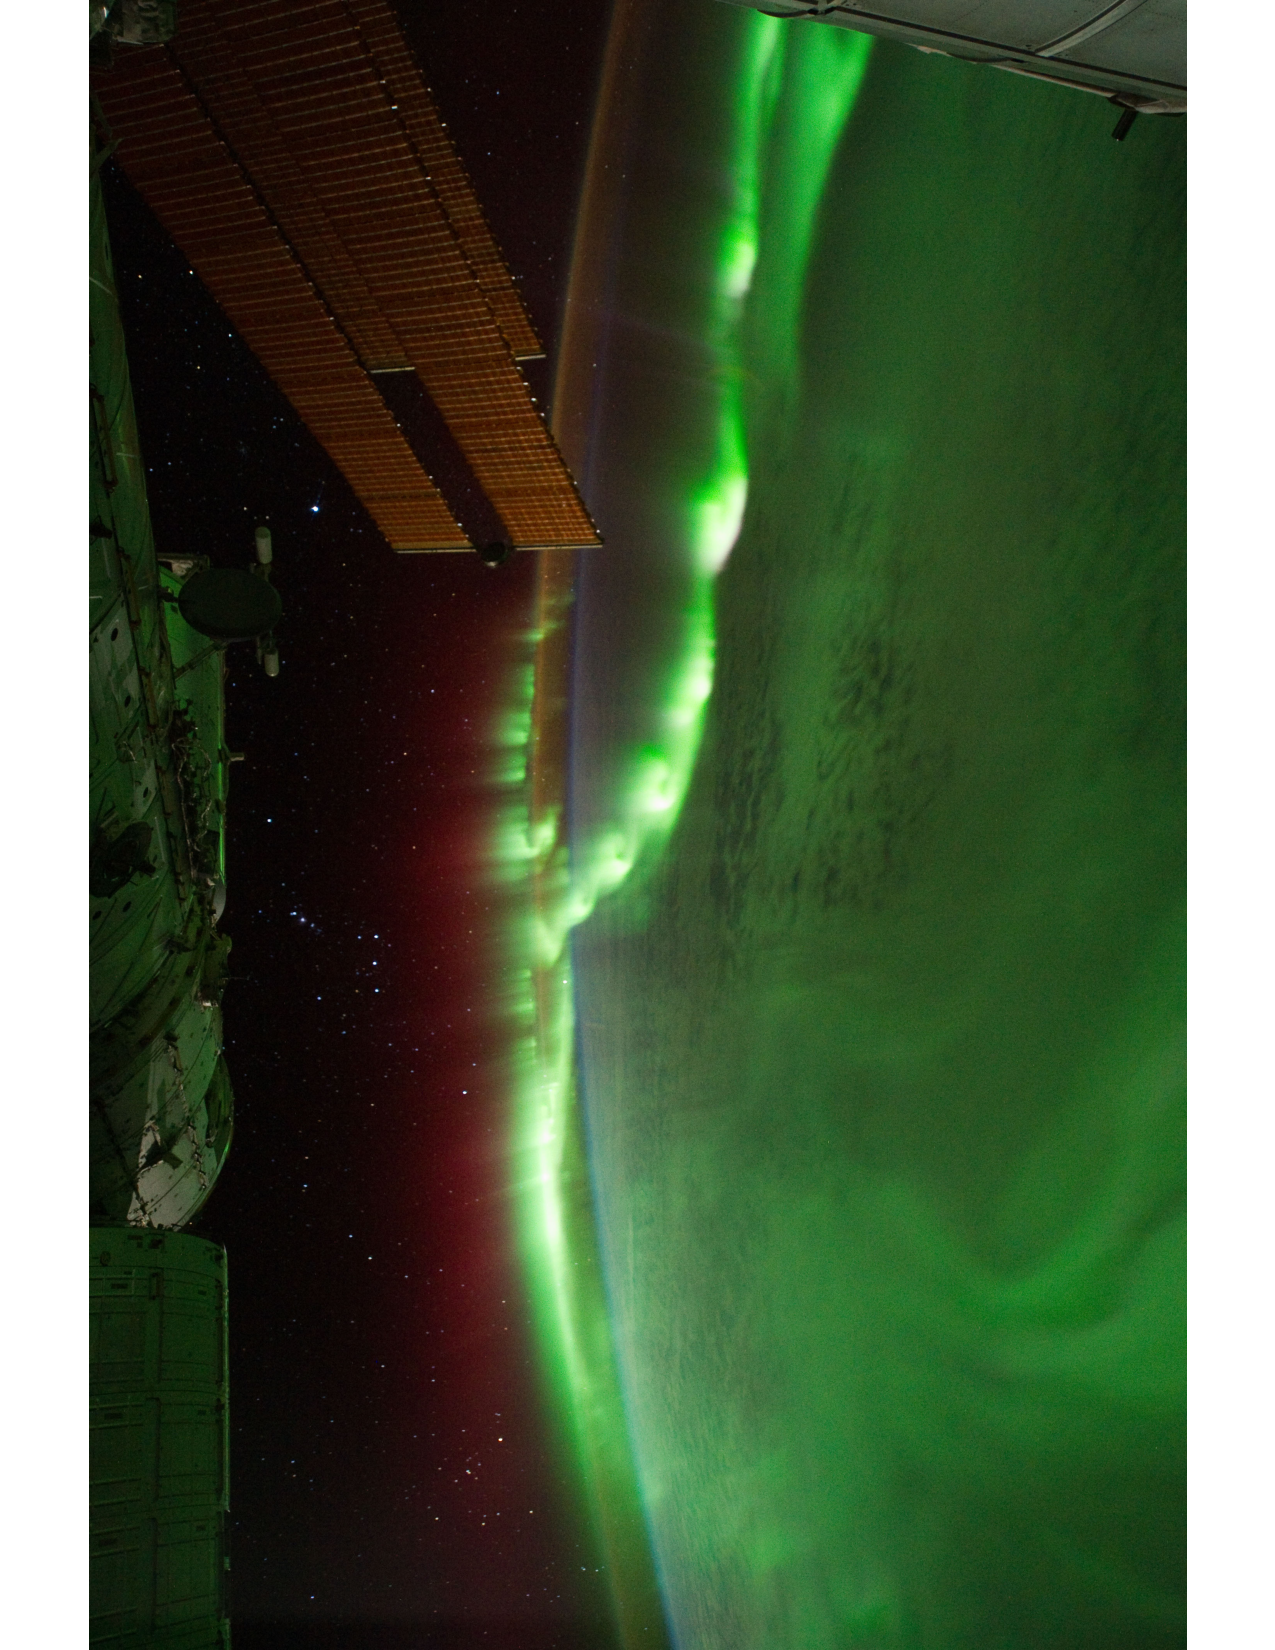
\includegraphics[width=.5\textwidth,angle=270]{figures/chapter_1/aurora_from_space/aurora_from_space}
\caption{This picture of the Aurora, taken from the International Space Station, shows that the space around Earth can have a lively and energetic character. Image by NASA, from nasa.gov.}
\end{centering}
\end{figure}

\section{The Earth's Atmosphere}

The atmosphere of the Earth has a structure, and this structure determines the environment where phenomena originating in space make most of their directly observable effects. The colours of the aurora, for example, are essentially determined by the wavelengths of light which the constituents of the atmosphere radiate when excited. Since the Earth's atmosphere is uniquely accessible to us, its structure is well known. We present a simple picture of the atmosphere which is sufficient for understanding the effects of energetic particle precipitation, discussed in the following chapter.

At the surface of the Earth, the atmospheric constituents are well-mixed. Most of the mass of the atmosphere lies in the region defined as the troposphere, which extends from ground level to to an altitude of around 10 kilometers. This dense region of the atmosphere is where life on Earth, and most terrestrial weather happens. The main structure of the troposphere is defined by a decrease in temperature and density with increasing height. Density decreases exponentially with altitude, which can be easily shown with the hydrostatic condition. Temperature is somewhat more complicated. Besides local effects (the weather), temperature decreasing with height owing to increased distance from the warm surface of the Earth. The lapse rate defines the rate at which temperature drops with height, and has a value of approximately 2 degrees C per kilometer of altitude. 

At the tropopause, the temperature of the atmosphere begins to increase with height. This is because near to the ground, the air is a fairly poor absorber of solar radiation. After the density of the atmosphere reaches a sufficiently low value, ultraviolet radiation causes the disassociation of molecular oxygen, which results in free oxygen atoms combining with diatomic oxygen to form ozone. Heat is a byproduct of this reaction. The next layer of the atmosphere, termed the stratosphere, begins here. The stratosphere is characterized by limited vertical mixing, and is very dry, with few weather effects from the troposphere reaching it. Winds in the stratosphere can be intense, reaching speeds of hundreds of 200 kilometers per hour depending on the region. The density in the stratosphere is low, ranging from a few percent of that at ground level to nearly zero at the vertical limit. The low density in the stratosphere makes it quite transparent to certain kinds of radiation from space. In particular, X-rays, created from the slowing down of charged particles farther up in the atmosphere, can propagate deeply in this region. This is where remote sensing of space effects based on secondary radiation becomes possible using balloon-borne instruments, discussed in the following section. 

At the end of the stratosphere, temperature once again begins to decrease with height. This occurs at an altitude of approximately 50 kilometers above the surface of the Earth. The mesosphere is the name given to this region of the atmosphere. Here, the different components of the atmosphere are still well-mixed owing to turbulence. This continues to be true to a height of around 80 kilometers. Meteorites burn up in this part of the atmosphere, and the temperature reaches a lower limit of approximately 100 degrees C at its highest point. Once the turbulent effects which occur in the mesosphere become less important, separation of the different atmospheric constituents occurs due to the different scales at which their densities decrease. The hydrostatic condition imposes exponential decreases in density with height, but the scale at which this happens depends on the particle mass. This gives rise to a structure in the upper atmosphere, with the proportions of the different components changes with height. This is important for modelling the propagation of  radiation, which has interactions which depend on the chemical composition, overall density, and temperature. 

Past the mesosphere lies a region called the thermosphere. In this region, climb sharply and then are steady with increasing height. Solar activity has a strong bearing on the temperatures in this region, which can reach hundreds or thousands of degrees C. Turbulant mixing no longer has meaning at the low densities in the thermosphere. The international definition of the beginning of space, a boundary that begins at 100 kilometers altitude, is contained in this region. In the thermosphere, the density begins to become sufficiently low that the rate of collisions between individual atoms and molecules becomes small enough to start treating them individually, rather than as a fluid. This is the domain where plasmas can exist, since ionized particles and electrons do not immediately collide and become neutral once they are created. This region of space is also called the ionosphere, for this reason.  Spacecraft orbit in the thermosphere; orbits with a practical decay time begin at heights of around 350 kilometers.

At heights of hundreds of kilometers, charged particles survive for long enough that electromagnetic interactions become important. Temperature takes on a different meaning, one based more on the statistical properties of individual and group particle motion, then the classical value that can be measured with a thermometer. The local magnetic field becomes the most important geometry and coordinate system, rather than the local vertical direction from Earth. Free from the dominating effect of collisions, particles undergo characteristic motions not seen in the lower regions of the atmosphere. In particular, they can interact with radio waves, both artificial and natural, and undergo collective motion that interacts with them. Figure~\ref{atmosphere_schematic} shows an illustration of some the different layers of the atmosphere, and how the population of charged particles changes with height.

It's not easy to draw a clear sharp line where the atmosphere ends. Such a definition probably needs to depend on the application or line of inquiry being pursued. For aircraft, heights past the stratosphere are unreachable owing to low density. Rockets can reach the intermediate heights between the stratosphere and the thermosphere, while orbiting satellites require further heights still, so that orbits decay on a sufficiently large timescale. Eventually, even the magnetic field of the Earth becomes less important than the magnetic field carried with the plasma of the solar wind, and farther past this point, the influence of the Earth and its magnetic field ceases. The exploration of the solar system, and beyond, by robotic spacecraft begins to  blur the distinction between space physics and astronomy. It is interesting, that the two fields are separated mostly by a practical limitation due to the vast distances involved, instead of a more fundamental, and natural boundary. 


\begin{figure}[p]
\label{}
\begin{centering}
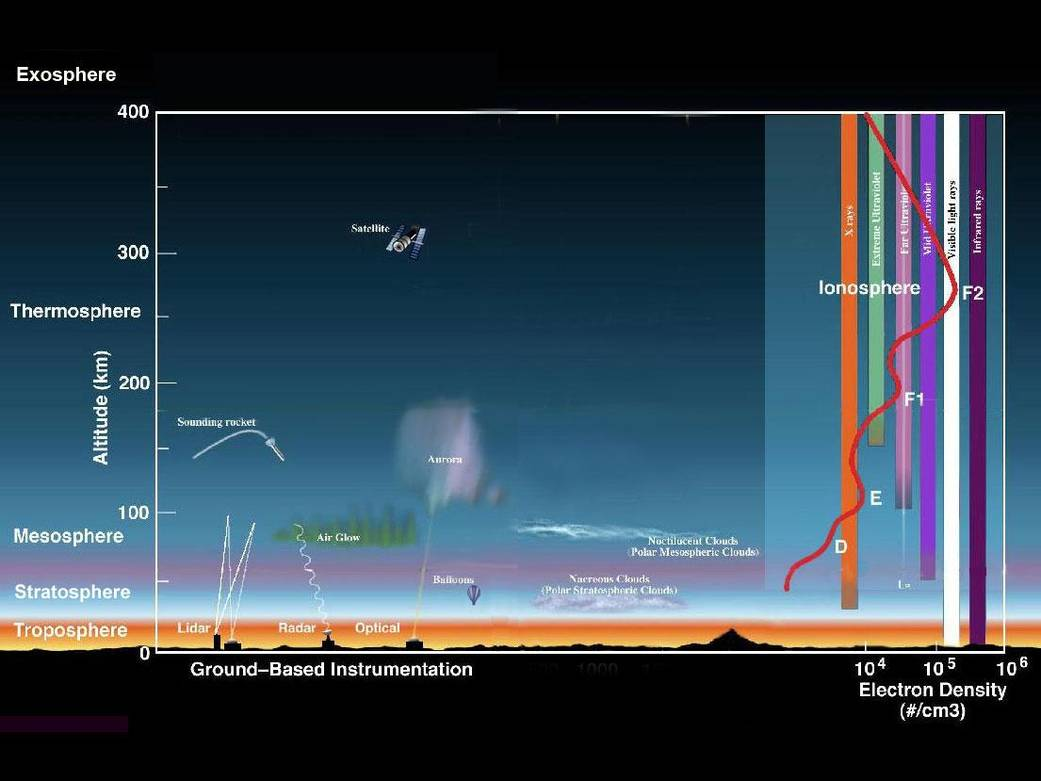
\includegraphics[width=.9\textwidth]{figures/chapter_1/atmosphere_schematic/atmosphere_schematic}
\caption{Schematic illustration showing the scale and structure of the atmosphere, with the overall trend in electron density with height. Image by NASA Goddard, from nasa.gov.}
\end{centering}
\end{figure}
\newpage

\section{Getting Above the Atmosphere with High Altitude Balloons}

Since the atmosphere shields most of the radiation from space, it is not possible to build ground-based experiments that are sensitive to X-ray and charged particle radiation. Rocket flights routinely reach heights where this is no longer a problem, but by their nature, the flight times are short, on the scale of minutes. Orbiting satellites are practical at altitudes far above where radiation from space deposits most of its energy, so there needs to be another kind of vehicle, to get instruments above most of the atmosphere by mass, and that can remain there for hours, or days.

Balloons are the vehicles used in this thesis to get above the shielding effects of the lower atmosphere, and measure radiation from space directly at altitude of 30 to 40 kilometers. High altitude balloons are large, thin, membrane structures, filled with either hydrogen or helium, which carry payloads ranging from grams to hundreds of kilograms, and ascend until they reach an equillibrium height in the stratosphere, which is above most of the radiation shielding effects of the atmosphere. Balloons need no external energy source to maintain their flight, and so can remain at altitude for hours, days, or even weeks depending on their design and the desired mission profile. With the exception of the balloons needed to carry the largest, heaviest, experiments, high altitude balloons are also inexpensive, compared with rocket flights and satellites. This opens possibilities for extensive surveys and coincident missions which do not exist when using other platforms. 

High altitude balloons follow two distinct designs. The first, called the zero-pressure balloon, is named because it maintains an internal pressure equal to the surrounding atmosphere. This is the type of balloon most frequently used for scientific experiments, because it has the property of passively remaining at peak altitude for extended periods of time. The design consists of a large polyethelyne bubble, with one or two vent ducts near the bottom, open to the atmosphere. The payload hangs beneath the balloon on a cable or rope. As the balloon is filled through the ducts, lift gas collects at the apex and causes hydrostatic lift. Once a predetermined amount of lift gas has been added, the balloon is released, and ascends, carrying the payload with it. As the balloon ascends, the internal lift gas expands to fill the balloon volume. Eventually, the balloon is completely filled with the low density lift gas, and excess is passively released through the vent ducts, causing the balloon to stop ascending and maintain a fixed altitude. When the balloon mission is terminated, cable cutting equipment is used to separate the payload from the balloon. The payload descends under parachute and is usually recovered. Upon release, it is typical that the payload rips a destruct panel from the balloon, causing it to release most of its lift gas and descend as well. The point at which this process happens is chosen in the design phase of the mission, and is typically activated by timer, remote command, or both. 

There is an ultimate limit to the flight duration which can be achieved using zero-pressure balloons, which is caused by internal temperature differences at day and night. During the day, solar radiation warms the balloon and the gas contained in it. When night occurs, the balloon begins to cool, which causes the gas inside to decrease in volume. The balloon has no rigid structure to maintain a fixed volume, so the balloon membrane then occupies less volume as well. This causes the balloon to start to descend. As the descent occurs, the surrounding atmosphere begins to increase in density. This reduces the volume of the balloon further, which causes more lift gas to be released through the vent ducts, which then increases the rate of descent. In practice, this feedback cycle is prevented through the controlled release of ballast, usually sand, on missions which need to extend for several days. It can be shown that the ultimate limit for the duration of zero pressure balloon flights is approximately 7 days, even if most of the payload consists of expendable ballast. The exception to this rule occurs for flights in the polar regions of the Earth, where the day night cycle is longer. Figure~\ref{zero_pressure_balloon_example} shows a zero-pressure balloon in flight, with the scientific payload being carried below.

\begin{figure}[p]
\label{zero_pressure_balloon_example}
\begin{centering}
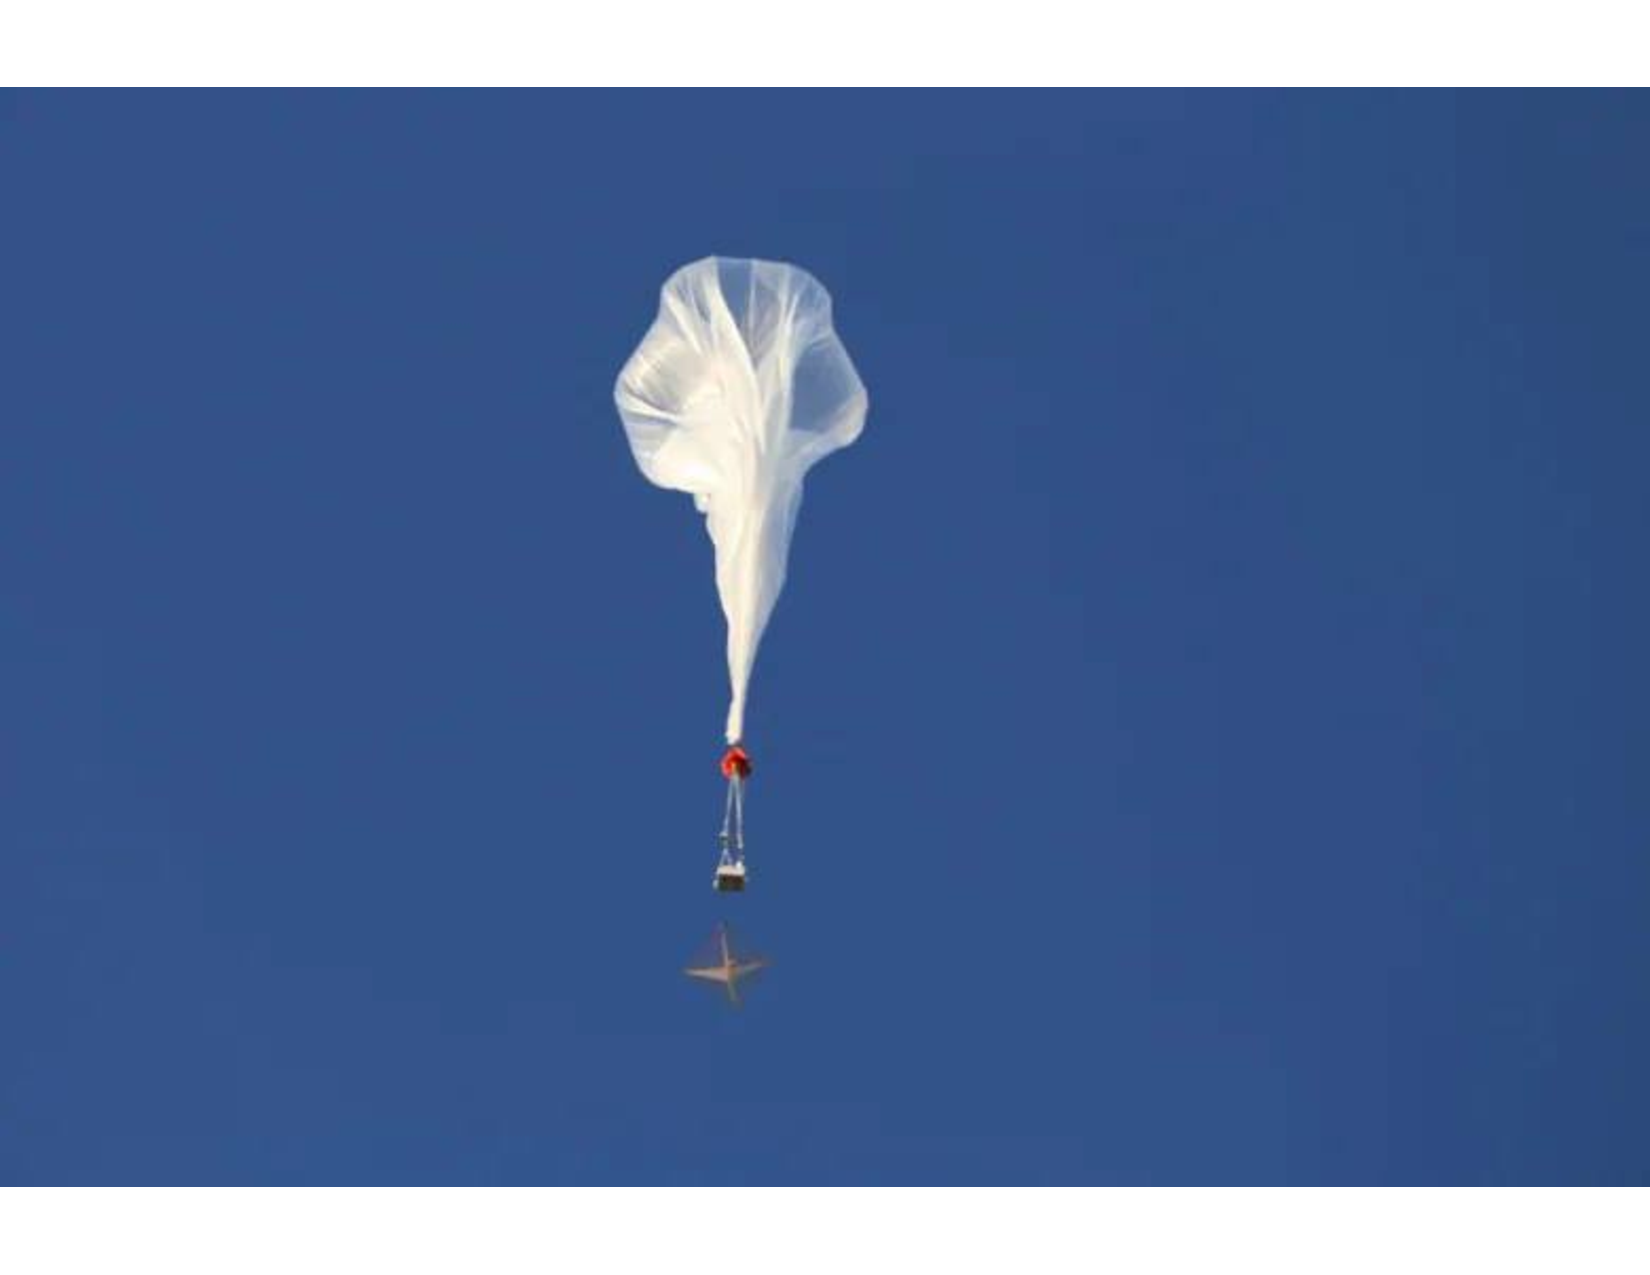
\includegraphics[width=.7\textwidth,angle=270]{figures/chapter_1/zero_pressure_example/zero_pressure_example}
\caption{Zero-pressure balloon in flight shortly after release. The lift gas will expand to fill the balloon volume during the ascent.}
\end{centering}
\end{figure}
\newpage

The second type of high altitude balloon is primarily used for meteorological experiments. Consisting of a relatively small latex sphere, this balloon is closed from the atmosphere and rises until the internal pressure causes it to rupture and descend. These meteorological balloons are launched regularly around the world several times per day to aid in the creation of weather models and forecasts. Typically carrying payloads of only a few hundreds of grams, to at most a few kilograms, these balloons reach heights comparable to the zero-pressure balloons, but do not maintain equillibrium altitude. This makes them less useful for the measurement of space radiation, although, some exotic ways to overcome this problem have been developed and tested (see Appendix 1). 


\section{Scope of this Thesis}

The question we ask in this thesis is: what is the maximum amount of information that can be obtained about processes far out in the space surrounding Earth, using measurements of the resulting radiation? High altitude balloons are a natural platform for the required measurements, and we will use several different flights to build up the required data set. These data will then be interpreted through a corresponding computer simulation of the environment, the detector, and the requisite mathematical analysis to form a picture of the process that extends from the emission of radiation from space, to the impact and measurement in the atmosphere. 

 


